\subsection{Client Connection}
\label{sub:eval:connection}


We define client connection as the amount of time it takes for a device to connect, as a client, to a published server.
This connection time takes into account not only the time it takes for that client to connect to the server, 
but also the time it takes for that client to have its own copy of the server state. 
To do so, we measured events related to client connection, server welcoming message, and the first message for that client that carried the server state.


Figure~\ref{fig:client-welcome} presents the cumulative empirical function for client connection.
On average, clients are fully connected to a publisher server in 11 seconds. 
The majority of the clients (80\%) were able to establish a connection under 15 seconds, 
but we noticed some cases were clients took longer to connect. 
Inspecting this corner case scenarios, we identified that they were mostly related to cases were the state was larger than 1MB.
In other cases were this affirmation did not hold, we hypothesize that the hotspot connection was not stable, but we lack data to support this hypothesis.


\begin{figure}
    \centering
    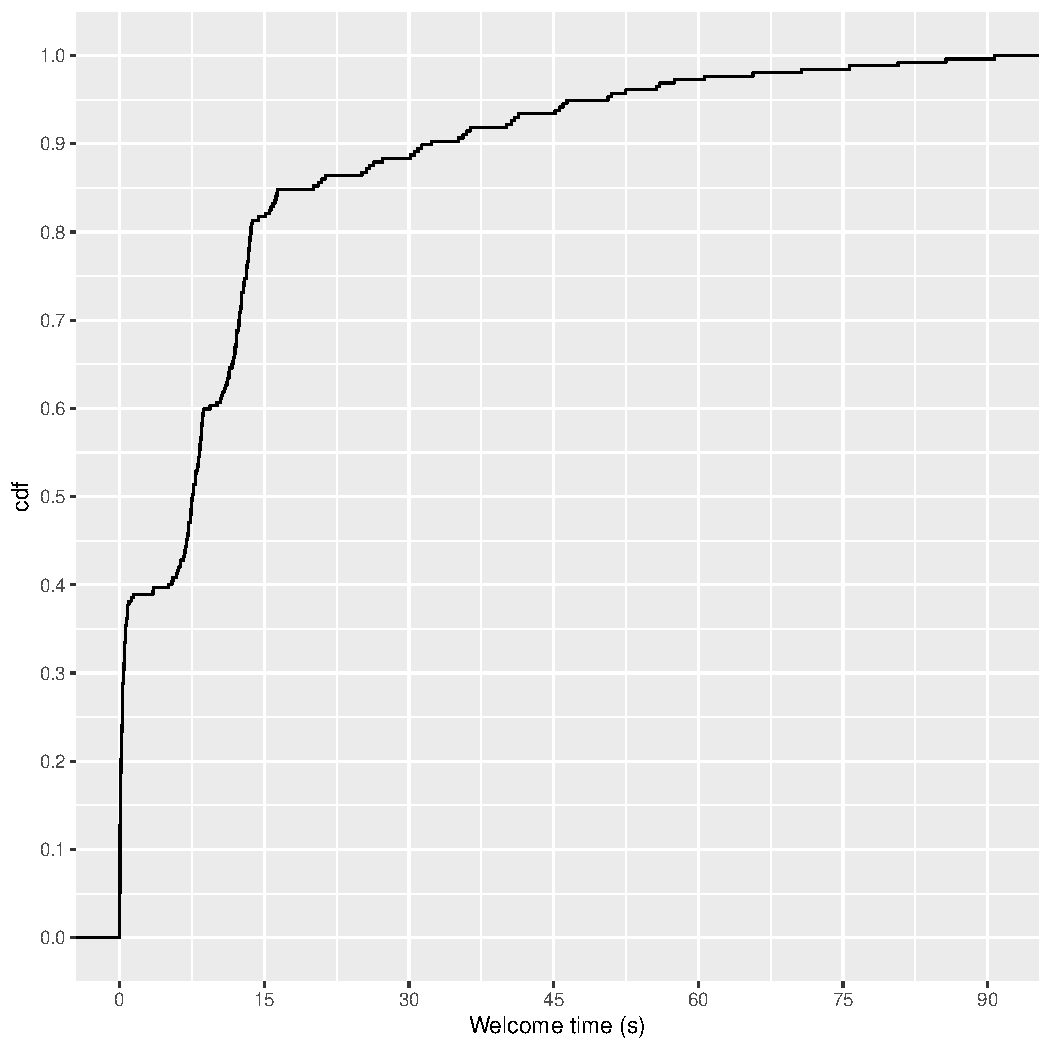
\includegraphics[width=0.9\linewidth]{client-welcome}
    \caption{Client time to open a connection and join the server until it receives the server state}
    \label{fig:client-welcome}
\end{figure}


In order to further investigate client connection properties, we investigate whether the number of connected devices or the server state size influences connection time.
Figure~\ref{fig:client-welcome-successors} presents a boxplot chat about the connection time grouped by the number of successors.
Despite the fact that all connected clients receive a state update with a new successorship list including the new connected client, 
we could not see how the number of successors influences a new client connection and all boxplot charts overlap.
On the other hand, Figure~\ref{fig:client-welcome-state-size} models time as a linear function of the server state size.
Intuitively, as the server state increases in size, clients take longer to connect. 


\begin{figure}
    \centering
    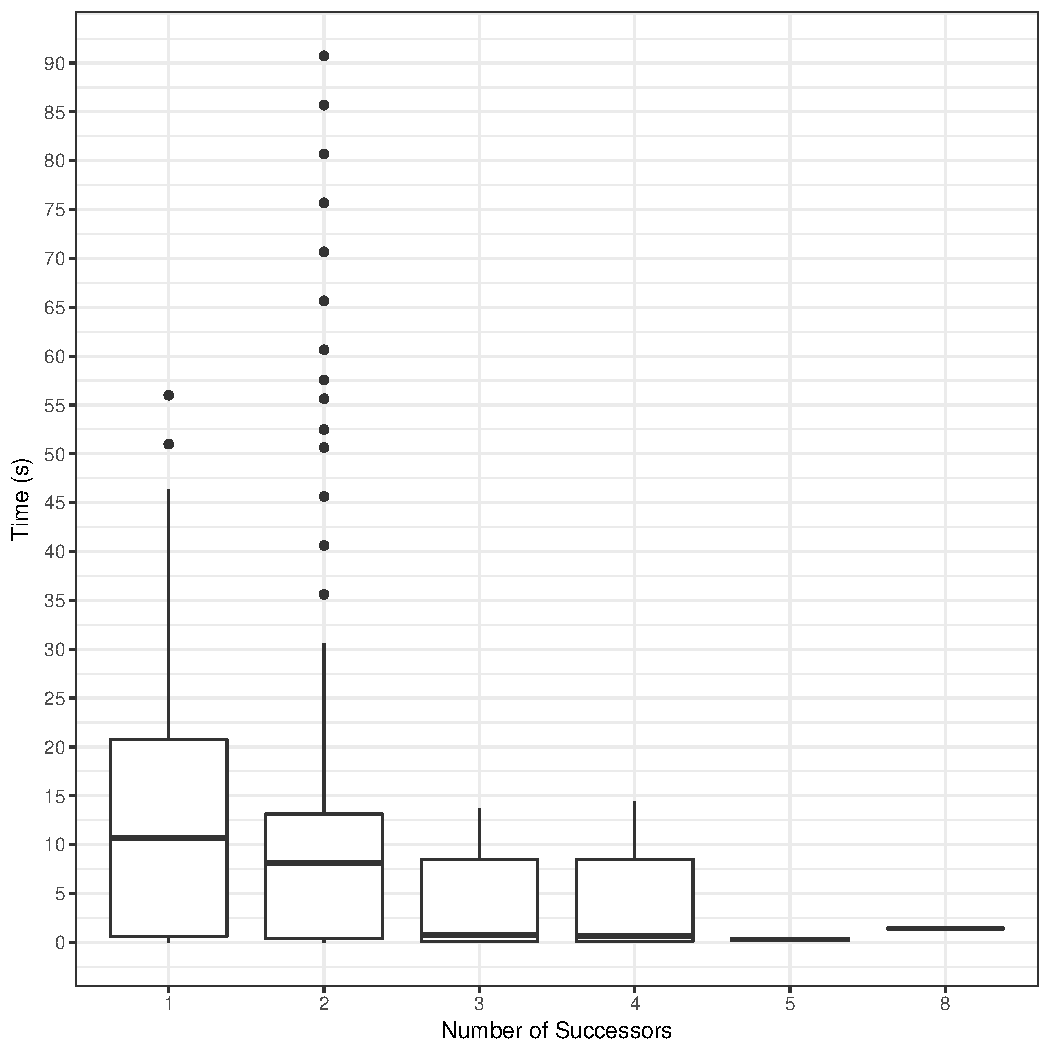
\includegraphics[width=0.9\linewidth]{client-welcome-successors}
    \caption{Client time to connect per number of successors}
    \label{fig:client-welcome-successors}
\end{figure}

\begin{figure}
    \centering
    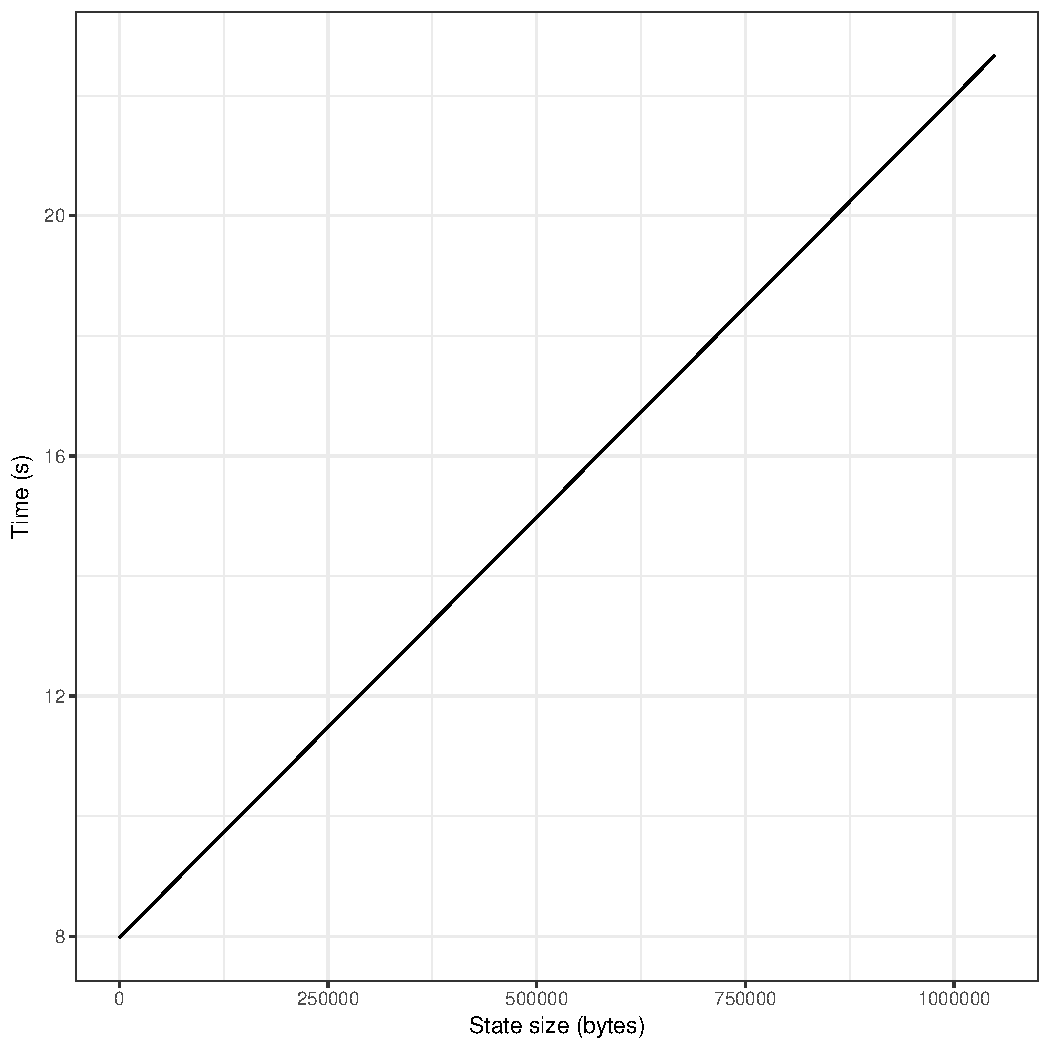
\includegraphics[width=0.9\linewidth]{client-welcome-state-size}
    \caption{Client time to connect as a function of the server state}
    \label{fig:client-welcome-state-size}
\end{figure}